\documentclass{sigchi}

% Use this section to set the ACM copyright statement (e.g. for
% preprints).  Consult the conference website for the camera-ready
% copyright statement.

% Copyright
\CopyrightYear{2021}
%\setcopyright{acmcopyright}
\setcopyright{acmlicensed}
%\setcopyright{rightsretained}
%\setcopyright{usgov}
%\setcopyright{usgovmixed}
%\setcopyright{cagov}
%\setcopyright{cagovmixed}
% DOI
\doi{https://doi.org/10.1145/3313831.XXXXXXX}
% ISBN
\isbn{XXX-X-XXXX-XXXX-X/21/05}
%Conference
\conferenceinfo{CHI'21,}{May 8--13, 2021, Yokohama, Japan}
%Price
%\acmPrice{\$99.90}

% Use this command to override the default ACM copyright statement
% (e.g. for preprints).  Consult the conference website for the
% camera-ready copyright statement.

%% HOW TO OVERRIDE THE DEFAULT COPYRIGHT STRIP --
%% Please note you need to make sure the copy for your specific
%% license is used here!
% \toappear{
% Permission to make digital or hard copies of all or part of this work
% for personal or classroom use is granted without fee provided that
% copies are not made or distributed for profit or commercial advantage
% and that copies bear this notice and the full citation on the first
% page. Copyrights for components of this work owned by others than ACM
% must be honored. Abstracting with credit is permitted. To copy
% otherwise, or republish, to post on servers or to redistribute to
% lists, requires prior specific permission and/or a fee. Request
% permissions from \href{mailto:Permissions@acm.org}{Permissions@acm.org}. \\
% \emph{CHI '16},  May 07--12, 2016, San Jose, CA, USA \\
% ACM xxx-x-xxxx-xxxx-x/xx/xx\ldots \$15.00 \\
% DOI: \url{http://dx.doi.org/xx.xxxx/xxxxxxx.xxxxxxx}
% }

% Arabic page numbers for submission.  Remove this line to eliminate
% page numbers for the camera ready copy
\pagenumbering{arabic}

% Load basic packages
\usepackage{balance}       % to better equalize the last page
\usepackage{graphics}      % for EPS, load graphicx instead 
\usepackage[T1]{fontenc}   % for umlauts and other diaeresis
\usepackage{txfonts}
\usepackage{mathptmx}
\usepackage[pdflang={en-US},pdftex]{hyperref}
\usepackage{color}
\usepackage{booktabs}
\usepackage{textcomp}
\usepackage{lipsum}

\usepackage{comment} %OSCARs insert

% Some optional stuff you might like/need.
\usepackage{microtype}        % Improved Tracking and Kerning
% \usepackage[all]{hypcap}    % Fixes bug in hyperref caption linking
\usepackage{ccicons}          % Cite your images correctly!
% \usepackage[utf8]{inputenc} % for a UTF8 editor only

% If you want to use todo notes, marginpars etc. during creation of
% your draft document, you have to enable the "chi_draft" option for
% the document class. To do this, change the very first line to:
% "\documentclass[chi_draft]{sigchi}". You can then place todo notes
% by using the "\todo{...}"  command. Make sure to disable the draft
% option again before submitting your final document.
% \usepackage{todonotes}

% Paper metadata (use plain text, for PDF inclusion and later
% re-using, if desired).  Use \emtpyauthor when submitting for review
% so you remain anonymous.
\def\plaintitle{The Pandemic Home Office For University Studies}
\def\plainauthor{First Author, Second Author, Third Author, Fourth Author}
\def\emptyauthor{First Author, Second Author, Third Author, Fourth Author}
\def\plainkeywords{distance learning; health; home office; motivation; pandemic; student;  study environment; work environment;}
\def\plaingeneralterms{Documentation, Standardization}

% llt: Define a global style for URLs, rather that the default one
\makeatletter
\def\url@leostyle{%
  \@ifundefined{selectfont}{
    \def\UrlFont{\sf}
  }{
    \def\UrlFont{\small\bf\ttfamily}
  }}
\makeatother
\urlstyle{leo}

% To make various LaTeX processors do the right thing with page size.
\def\pprw{8.5in}
\def\pprh{11in}
\special{papersize=\pprw,\pprh}
\setlength{\paperwidth}{\pprw}
\setlength{\paperheight}{\pprh}
\setlength{\pdfpagewidth}{\pprw}
\setlength{\pdfpageheight}{\pprh}

% Make sure hyperref comes last of your loaded packages, to give it a
% fighting chance of not being over-written, since its job is to
% redefine many LaTeX commands.
\definecolor{linkColor}{RGB}{6,125,233}
\hypersetup{
  pdftitle={\plaintitle},
% Use \plainauthor for final version.
%  pdfauthor={\plainauthor},
  pdfauthor={\emptyauthor},
  pdfkeywords={\plainkeywords},
  pdfdisplaydoctitle=true, % For Accessibility
  bookmarksnumbered,
  pdfstartview={FitH},
  colorlinks,
  citecolor=black,
  filecolor=black,
  linkcolor=black,
  urlcolor=linkColor,
  breaklinks=true,
  hypertexnames=false
}

% create a shortcut to typeset table headings
% \newcommand\tabhead[1]{\small\textbf{#1}}

% End of preamble. Here it comes the document.
\begin{document}
\title{\plaintitle}
\numberofauthors{4}


\author{
    Andreea-Valentina Roman\\
    \affaddr{Vienna University of Technology}\\
    \affaddr{Vienna, Austria}\\
    \email{e12019805@student.tuwien.ac.at}
    \and
  Dragos-Alexandru Gabor\\
    \affaddr{Vienna University of Technology}\\
    \affaddr{Vienna, Austria}\\
    \email{e11932446@student.tuwien.ac.at
}
 \and
Joanna Zamiechowska\\
    \affaddr{Vienna University of Technology}\\
    \affaddr{Vienna, Austria}\\
    \email{e11936038@student.tuwien.ac.at}
 \and
Oscar Larsson\\
    \affaddr{Vienna University of Technology}\\
    \affaddr{Vienna, Austria}\\
    \email{e12015240@student.tuwien.ac.at}

}


\begin{comment}
\author{
  Andreea Roman\\
  \affaddr{Vienna University of Technology}\\
    \affaddr{Vienna, Austria}\\
    \email{e12019805@student.tuwien.ac.at}
  \and
  Dragos-Alexandru Gabor\\
  \affaddr{Vienna University of Technology}\\
    \affaddr{Vienna, Austria}\\
    \email{e12019805@student.tuwien.ac.at}
    \AND
  Dragos-Alexandru Gabor\\
  \affaddr{Vienna University of Technology}\\
    \affaddr{Vienna, Austria}\\
    \email{e12019805@student.tuwien.ac.at}
    \and
  Dragos-Alexandru Gabor\\
  \affaddr{Vienna University of Technology}\\
    \affaddr{Vienna, Austria}\\
    \email{e12019805@student.tuwien.ac.at}
}
\end{comment}

\maketitle

\begin{abstract}
Given the appearance of the new pathological risk incurred during the COVID-19 pandemic, most educational institutions, be they either lower or higher education, have had to restrict their on-campus activities and promote a fully online pedagogical approach in order to avoid the spread of the virus and protect the health of both students and teachers. By employing already existing software solutions facilitating video streaming (e.g. Zoom) and course management (e.g. Moodle), courses have, in most cases, been completely moved into the realm of the internet to the best of the ability of each educational institution. In this context, we are trying to investigate the effects that the sudden move to distance learning has had on students of different backgrounds, as well as how they have been forced to change their study and work environments to cope with the perpetual stress of academic life within the confines of their own home. After analyzing eight different student situations, there are indications that many students have a lower level of motivation in the current distance learning format. The technical equipment is upgraded but not always fully complete. There is still a majority who are not satisfied with their home office furnishings, mainly the office chair. However, there seems to be a lack of awareness of how simple ergonomics can be improved, partly because the student has downgraded this priority in the hope of soon returning to normal campus studies. Financial limitations are also a constraint.
\end{abstract}

%Not to use, repetitive: The equipment varies depending on the student and situation.

% ACM Classfication
\begin{CCSXML}
<ccs2012>
<concept>
<concept_id>10003456.10003457.10003527.10003542</concept_id>
<concept_desc>Social and professional topics~Adult education</concept_desc>
<concept_significance>500</concept_significance>
</concept>
<concept>
<concept_id>10003120.10003121</concept_id>
<concept_desc>Human-centered computing~Human computer interaction (HCI)</concept_desc>
<concept_significance>500</concept_significance>
</concept>
<concept>
<concept_id>10003120.10003121.10003122.10003334</concept_id>
<concept_desc>Human-centered computing~User studies</concept_desc>
<concept_significance>100</concept_significance>
</concept>
</ccs2012>
\end{CCSXML}

\ccsdesc[500]{Social and professional topics~Adult education}
\ccsdesc[300]{Human-centered computing~Human computer interaction (HCI)}
\ccsdesc[100]{Human-centered computing~User studies}

% Author Keywords
\keywords{\plainkeywords}

% Print the classification codes
\printccsdesc

\section{Introduction}

At the start of 2020, most countries around the world have had to impose strict restrictions upon public spaces and institutions in order to combat the eventual spread of COVID-19 within their population. One measure imposed upon the educational system was to forbid as much as possible lectures and other educational activities within their campuses as to avoid unnecessary and possibly life-threatening contact between students and members of the institution. In order to continue with the already started semester, most if not all education institutions have put forward online procedures based on existing infrastructure in order for the courses to still take place. Consequently, students have suddenly found themselves studying full-time from their homes, no longer allowed to study in libraries, cafes, or at the university campus. \\

Not being able to study on campus as a student can be frustrating as well as challenging. A study from 2002 showed that "e-learning" was so challenging that approximately 80\% of those who participated in such a course would fail \cite{1}. Today, almost 20 years later, the circumstances have changed. Over the past 20 years, technology has developed radically and have improved conditions for how distance-based studies can be conducted. Since the turn of the millennium higher education institutions have had the opportunity to expand large parts of their functions with digital solutions \cite{2}. Offering distance learning not only improves students' study conditions but also allows better opportunities for the university to remain international, future-oriented, and profit-driven \cite{2}. For example, a university that offers distance learning attracts more students from other locations, nationally as well as internationally. Digital solutions in terms of online procedures and digital learning platforms are fundamental to the university's modern infrastructure, although this internal infrastructure has not previously been tested for a complete shift to distance learning during a pandemic. \\

We, the research team of this conference paper, have also noticed certain trends of our own study behaviour during the distance learning semesters in Summer 2020 and Winter 2020. We have become aware of rising motivational issues due to distance learning. However, there is still an uncertainty as to whether this is true for the majority of the student population, and how unique situations may affect home learning. Hence, the following conference paper will perform an inquiry under a practice research study for the course \textit{193.056 User Research Methods Project} at Vienna University of Technology, Austria, in order to investigate this issue. The research study will examine if there is a general unpreparedness across the student population for such a drastic move to distance learning, as well as if there is such a notion as a \emph{``perfect study environment or study setup''}. This research result will help us compile recommendations for both students and educational institutions, which aim to help reduce the amount of stress caused by social isolation and full-time distance learning, and increase students' acceptance of the distance learning situation \cite{fauci_lane_redfield_2020, hossain_mental_2020}.

%HCI, do we need more of this in this paper?

\section{Related Work}

The following paper is related to a British motivation research study that examined the basic factors that influence successful distance learning \cite{simons_leverett_beaumont_2019}. The research established how the students' knowledge and autonomy relate to the inherent motivation in a distance-adapted study environment, and how the educational institution may affects this result. It should be added that this research was conducted before the COVID-19 pandemic and therefore describes a distance learning situation that differs from the current situation. However, the research identifies various factors that affect the students' results in a distance learning setting. We believe that continuously supporting the student is a fundamental factor for a successful outcome. This applies not only for universities but also for family, friends, and employers. Feedback needs to be adapted to each student. Communication should take place with one-to-one contact. Supporting the student means that the student is more likely to make conscious choices in their studies. Another important aspect is flexibility and the need to be able to adapt the studies depending on the students' needs. For example, accessing study materials online can be a form of flexibility. Consequently, intrinsic motivation consists of an interplay between support and flexibility, which should be taken into account when investigating this topic.

Preceding all research methodologies, we conducted other literature reviews related to distance learning, home office studies, social isolation, and previous HCI related papers connected with the overall theme of the research questions and the methodologies used in our research. Four papers have been identified as either approaching the notion of distance learning motivation and competencies \cite{kolodziejczak_roszak_2017, simons_leverett_beaumont_2019}, students' preferred learning environments \cite{beckers_voordt_dewulf_2016}, or other works related to the impact that office comfort has on productivity \cite{sakellaris_et_al._2016}. 

Using \emph{Google Scholar} and the search inputs containing \emph{distance learning}, \emph{pandemic}, \emph{study environment}, \emph{COVID-19}, close to none have been found on the specific topic of the 2020 pandemic influences on distance learning, likely due to it being the first ever moment in human history that an epidemiological issue of this proportion has been encountered in the age of the internet, allowing the possibility of partaking in educational activities without putting one's life at risk. In the most relevant paper found, Lovric et al\cite{Lovri__2020}, the researchers performed an analysis on nursing students' perception of their overall experiences while studying during the COVID-19 pandemic, highlighting students' increasing worries and preference that educational institutions extend the already ongoing distance learning procedures.

Upon reviewing different research methodologies and scientific papers through the course \emph{193.055 User Research Methods}, the authors have decided to proceed with a research strategy involving auto-ethnography, semi-structured interviews, and photographic ethnography\cite{adams_ellis_jones_2017, adams_2015, douglas_2003, schwartz_visual_1989} considering these methodologies as being the most appropriate, and capable of creating a coherent strategy for the short amount of time and resources available. 

\section{Methods}

The following section will describe the research question, as well as the methods used in the research study, to show how these methods are integrated with each other in order to create a research strategy.

\subsection{Research Questions}

A distinct but primitive research question was designed to guide the research. The fundamental idea of the research question was to \textit{investigate how the home environment of the university student has changed to accommodate full-time study under the restrictions of the COVID-19 pandemic}. In order to answer this main research question, it was broken down into two more concrete secondary research questions, which would explore \textit{how the location of the study area has changed}, as well as \textit{how the equipment of the study area has changed}. 

\subsection{Methodologies}
In order to perform the research as best as possible, we decided on utilizing three separate methodologies in order to achieve a coherent approach and take into account various aspects related to the \emph{study environment}. We started by performing auto-ethnography upon ourselves to have an introspective look over our own experience during the first and second semesters of our studies within the context of the pandemic restrictions. Using the findings of the auto-ethnography, we arrived at a number of interview questions that where used in a series of semi-structured interviews with participants outside of the research team. Lastly by performing a photographic ethnography of the pictures taken by the same interview participants in order to analyse them in parallel with the interview transcriptions, a more coherent image of each participants' actual study environments is achieved. The following sections will explain which methods are used and our overall methodological strategy.

\subsubsection{Auto-ethnography}

The research began with the auto-ethnography \cite{adams_ellis_jones_2017, dighe_joshi_2014} approach. Each researcher conducted an inner-inquiry upon their experience that resulted from the drastic change to full-time distance learning, as well as making a comparison between their study/work environment and their study workload between previous semesters.

Upon finishing our reports on our own experience, each researcher had to take a photograph of their current study environment (see Figure~\ref{fig:figure1} as an example) and attach it to their report. Afterwards all reports where analysed by each researcher and the researcher-participant had to present their experience to the team. The information was then analysed using \emph{thematic analysis} within \emph{Miro}\footnote{\url{https://miro.com}} so as to extract possible interview questions for later use. After having decided on the possible interview questions, a practice semi-structured interview took place, with one of the researchers as a participant, and two others as interviewer and observer. Upon finishing the sample interview, the interview questions were refined down to five central questions that were used as a guide for the participant interviews.
\begin{figure}
\centering
  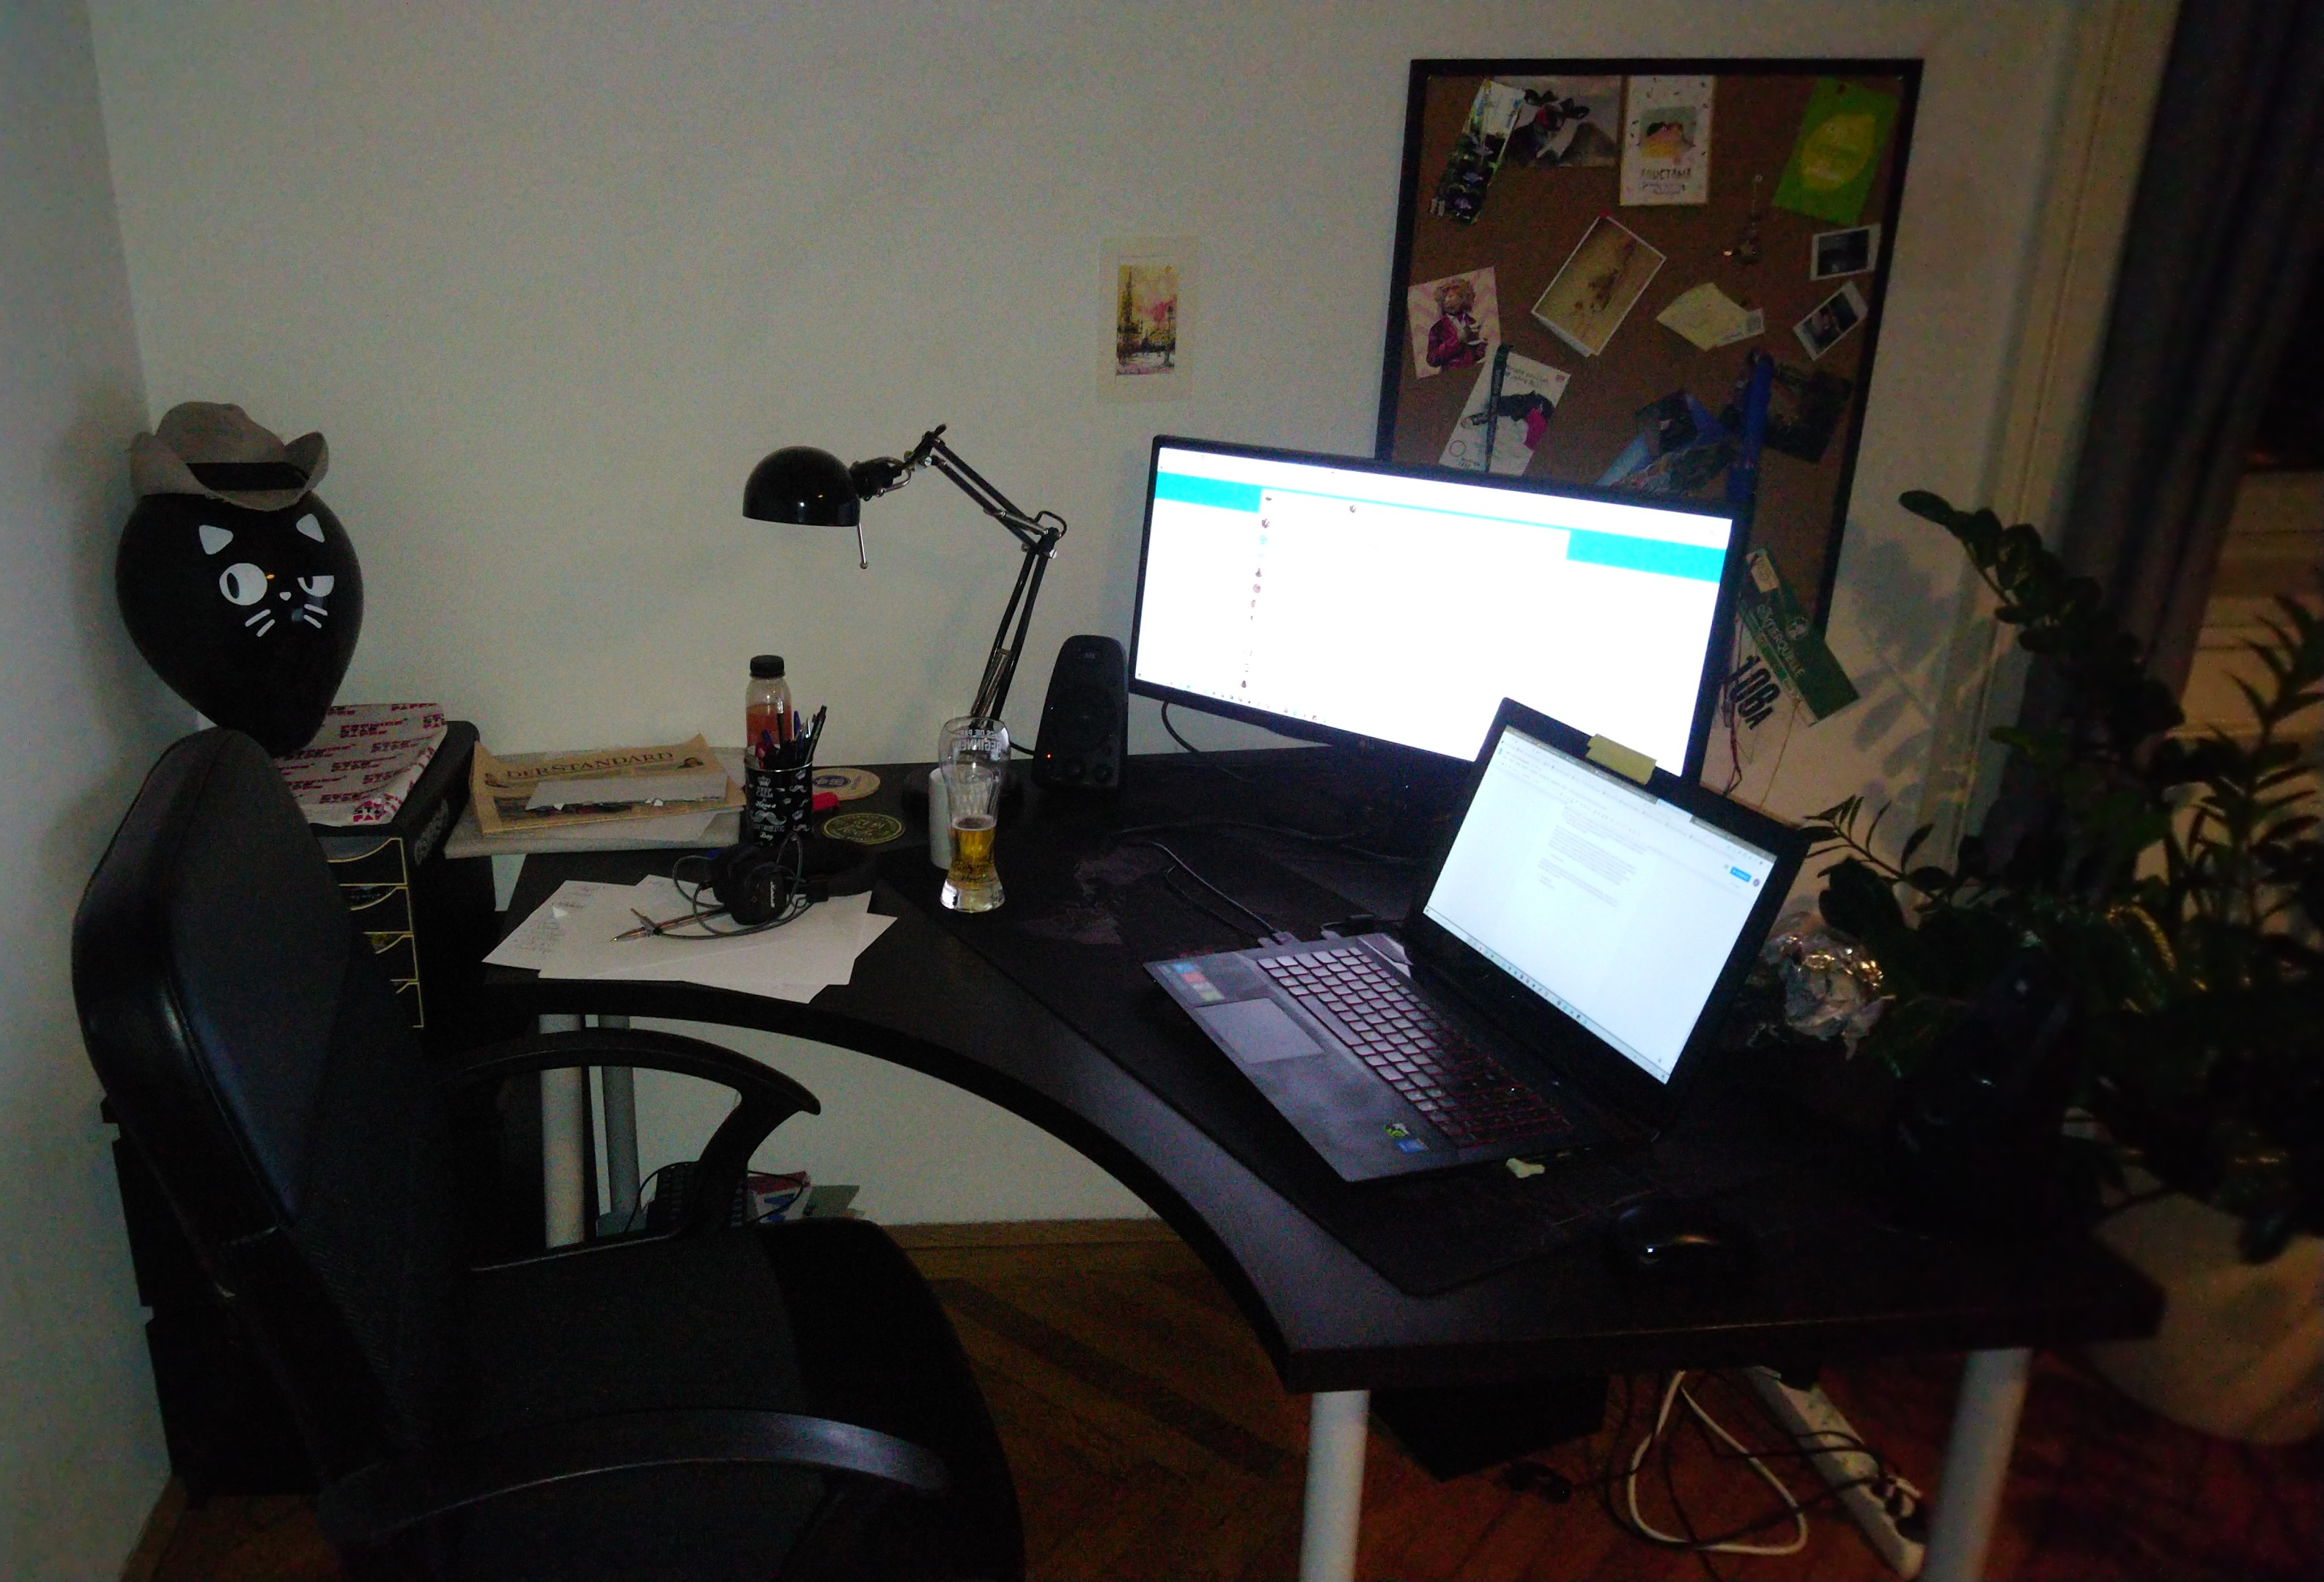
\includegraphics[width=1\columnwidth]{figures/auto-ethnography.JPG}
  \caption{Sample photograph from the auto-ethnographic method, showing the desk of one of the researchers}~\label{fig:figure1}
\end{figure}

\begin{figure}
\centering
  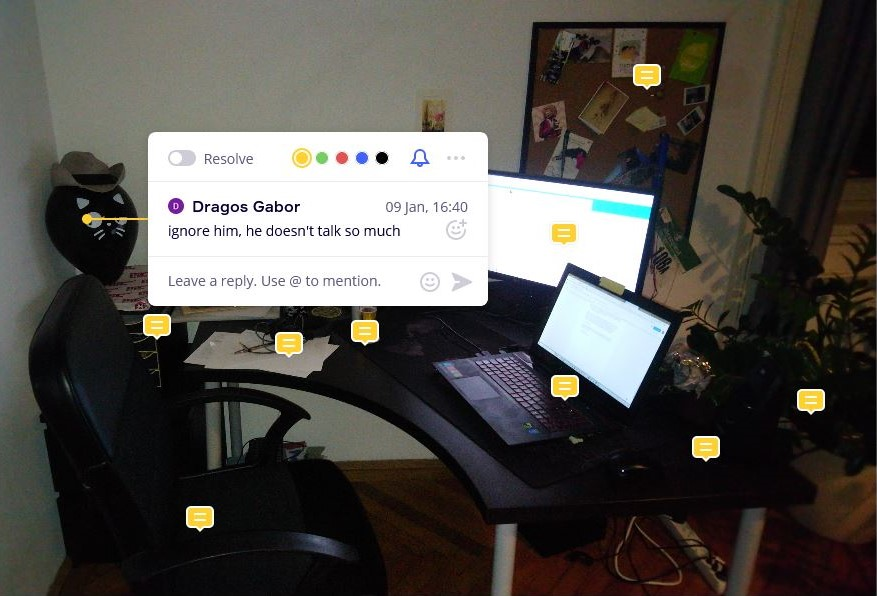
\includegraphics[width=1\columnwidth]{figures/auto-ethnography-annotated.JPG}
  \caption{Applying annotation to the same photograph as shown in Figure \ref{fig:figure1}}~\label{fig:figure2}
\end{figure}

\subsubsection{Semi-structured Interviews}
Semi-structured interviews\cite{adams_2015} were conducted to gather more information on how the home studying environment had changed for a variety of students. We opted for this more open style of information gathering because of the diverse variety of possible living situations. 

Our participants were friends and colleagues from varying backgrounds, countries, universities, and degree programs. An overview of their basic information is shown in Table \ref{tab:table1}. Using our interview questions as a guide to prompt a discussion on a specific point of interest, the semi-structured format allowed us to ask follow-up questions to further explore the participants' unique situations. These details may not have been captured in a more strictly structured interview or by a survey.

The topics that guided our interview questions centered on the home and study-area environment. First we asked questions to determine their current student and work status in order to get an idea for how heavy their work-loads were. This helped us understand how intensely they use their home office, and how important it is for their work and studies. We also asked questions about their living situations to understand how they might deal with issues of privacy, noise or other distractions, and sharing study-spaces with cohabitants. We then asked about their study-area and immediate surroundings. This gave us a picture of their immediate study environment; what equipment they use and how they use the space. We also asked them to think about the semester before the pandemic, and to reflect upon any changes they made to their study areas since transitioning to full-time distance learning. This includes rearranging furniture, purchasing or upgrading new equipment, or using old things in new ways. We then asked about any issues or challenges present in their current studying environment. Finally we asked them to imagine their ideal study area, and to share any improvements or "wish-list" items they would like if they could change anything and afford to do so. 
\begin{table}
  \centering
  \begin{tabular}{l l l l}
    % \toprule
    & & \multicolumn{2}{c}{\small} \\
    \cmidrule(r){1-4}
    {\small\textit{ID}}
    & {\small \textit{Academic Program}}
      & {\small \textit{Living Space}}
    & {\small \textit{Study Space}} \\
    \midrule
    P1 & Bio-Med Engineering & Shared Apt. & Bedroom \\
    P2 & Interaction Design & On-Campus & Shared Dorm \\
    P3 & Mechatronics & On-Campus & Shared Dorm \\
    P4 & Physics & Shared Apt. & Bedroom \\
    P5 & Data Science & Shared Apt. & Bedroom \\
    P6 & PhD Law & Apartment & Living-room \\
    P7 & Data Science & With Parents & Bedroom \\
    P8 & Artificial Intelligence & With Parents & Bedroom \\
    % \bottomrule
  \end{tabular}
  \caption{A variety of living and studying situations}~\label{tab:table1}
\end{table}

The participants were invited to take part in a short interview of approximately 30 minutes to discuss their current home studying environment, and to compare it with a semester before the pandemic. They were given information sheets and consent forms, informing them that their identities would remain anonymous to all but the interviewer and the consent form manager. They were also asked to provide a photograph of their studying area for photographic ethnography.

To avoid risk of COVID-19 exposure to both participant and researcher, all interviews were conducted via video conferencing and recorded with consent from the participant. The researcher then transcribed the recordings using \emph{Temi}\footnote{\url{https://www.temi.com}}. The transcriptions were finally anonymized and shared with the team for analysis. We then applied thematic analysis to the content of the transcripts on a shared Miro board. The themes and patterns that emerged are discussed in the Findings section.

\subsubsection{Photographic Ethnography}
Using the photographic ethnography method, we attempted to study the home study spaces of participants in more detail. The method was chosen in order to give a better overview of essential items used by students for improving their health and comfort during online studies at home. The participants agreed on sending a photograph of their study environment before the semi-structured online interviews in a email to the researcher who provided the consent forms. Moreover, the photographs of the researchers' personal setups, provided in the auto-ethnography phase, were also analyzed. The processes of storing, analyzing, anonymizing, and deleting the participants' and researchers' photographs were covered in the consent forms signed for the semi-structured online interviews and for auto-ethnography.

As visual recording of one's personal space can be considered a breach of privacy. Not all the participants agreed to photograph their study areas. In all, 21 photographs were collected in the photograph ethnography process. Some participants sent multiple photographs of their desk from different perspectives. A visual comparison between the state of the learning environment before and after switching to distance learning could not be made, as the photographs received were taken in the current context of the pandemic. One participant sent a photograph of their current setup, and two pictures of their ideal study space that could serve as inspiration for their future office arrangement (see Figure~\ref{fig:figure3}\cite{instagram_2019}). All photographs received by the participants were used in the analysis process.

The photographic ethnography method was used as an independent method to make a classification of the items used by students in the distance learning process, but also as a complementary method for the semi-structured interviews, to help us in having a more clear visualization of the environments of the participants. After collecting and anonymizing all the visual data, we arranged the photographs in Miro by a color and number code scheme. Every photograph would have the same number and color as the interview notes, which made sure we analyzed the transcripts of the corresponding photographs. This method of classification was used to offer a better correlation between the described environment and the representative photograph.

For an easier understanding of one's home study area, the photographs sent by us were completed with short annotations on objects present in the image (see Figure \ref{fig:figure2}). Each note summarized what the specific object is, what it is used for, and how it improves the quality or efficiency of the distance learning process.

\begin{figure}
\centering
  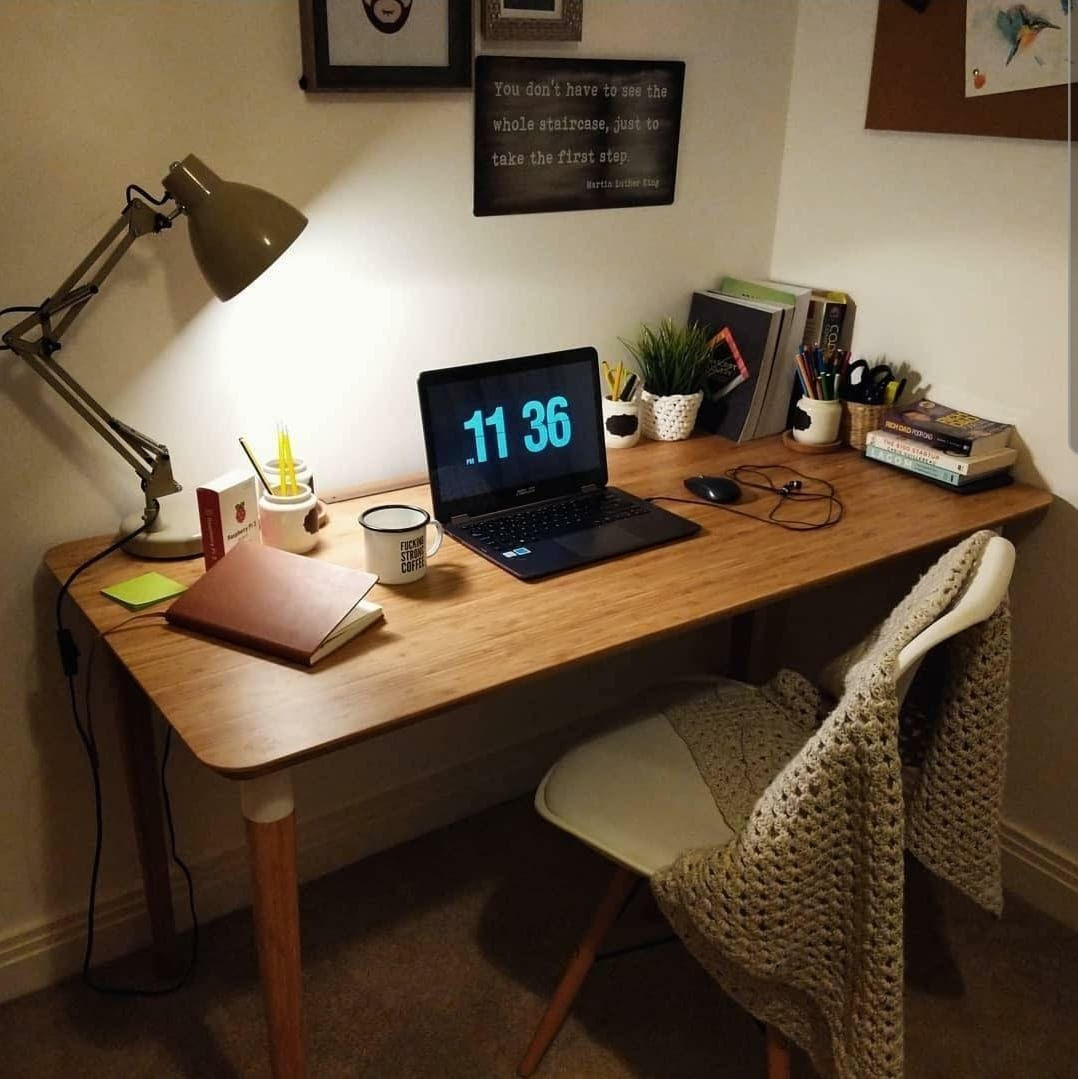
\includegraphics[width=1\columnwidth]{figures/perfect-setup}
  \caption{A sample picture from the Photographic Ethnography method given by one of the participants; it shows the desired \emph{perfect study environment}}~\label{fig:figure3}
\end{figure}

\section{Findings}

\subsection{Auto-ethnography}
Every researcher that took part in the auto-ethnographic process is currently taking part in distance learning, differing in degree program and the number of credits per semester. Some researchers admitted to registering for more courses this semester than in a typical, on-campus semester. The rationale was that commuting to the university is no longer required, and activities outside the house are restricted by the current regulations, which frees up more time for coursework. One participant admits that they overestimated the extra time that could be gained from not commuting, traveling, or taking part in social activities. Every researcher had to implement changes in their everyday schedule and their way of working on group projects or individual assignments, in order to respect the regulations in place caused by the pandemic:

\begin{quote}
\emph{All the projects I was doing at home, inviting colleagues over, at their place or in a coffee place. Now all the meetings are remote.}
\end{quote}

All researchers made changes to their home study setup. One participant who received an ergonomic desk and an additional monitor from their employer focused more on improving the room aesthetics, decorating with plants and drawings, and painting their wall. They mentioned that creating a comfortable, cozy place improves efficiency during working time. Another participant changed the location of their study area from a common room to a guest room that is no longer being used due to the restrictions. This change in location was to avoid being disturbed in the common room. 

All researchers want to improve their current study area as the distance learning may extend into the future. Common items that are desired for creating a more effective study space are ergonomic chairs, adjustable height desks, better headsets, second monitors, desk lamps, or even separate working/studying places at home. 

\subsection{Semi-structured Interviews}
After transcribing the recorded interviews, we read each-others' transcripts and analysed them. Using thematic analysis we identified some emerging themes. The most common themes were disruptions and annoyances in the home, complaints about poor ergonomics that resulted in pain, the importance of lighting, and strategies to maintain focus and motivation.

We found that all but one student made changes or improvements to their home study environment. This student still attends lectures on-campus, but at reduced capacity. The frequency with which they study at home has not notably increased since the pandemic. Equipment upgrades included purchasing a printer and scanner, improving lighting, new headsets or noise-cancelling headphones, a laptop stand, a power strip, new house plants, and lumbar support to prevent back pain. Some changes that did not require spending any money include moving furniture to create a more separate dedicated study area, moving desks closer to a window for better lighting, and using a whiteboard that went previously unused. 

We found that even if sharing a home with other people, most participants now have a dedicated study area where they can be alone, where before they had to share their study space with others or study in a common area. The exception are the students who live on-campus in a dormitory. 

In most cases the desk and study area is in the bedroom. This combination of study and sleeping space was sometimes a problem for some participants. One participant said it was difficult to take breaks and relax because they were surrounded by reminders of work, where when they were attending lectures on-campus there was enough of a separation to make the switch mentally. Some students combat this by making a point to do all school-related work only at the desk, where before they might have done some studying on the couch, in a chair, or in bed.

Some people were initially reluctant to make changes or invest money because of the uncertainty about how long the pandemic restrictions will remain in effect. At the time of this writing, we are currently in our second distance learning semester. While most of the changes discussed by our participants were enacted in their first pandemic semester, some larger purchases finally were made during the second pandemic semester.  

Lastly we asked how their ideal setup would look like if they could make further changes or investments. The most common ``wish-list'' item was a more comfortable chair. Students are spending sometimes over 12 hours in their chairs. Reports of back pain were the most common complaint among our interviewees.

\subsection{Photographic Ethnography}
We analyzed 11 sets of photographs both from the participants involved in the interview and from ourselves. We found that every student has a dedicated study setup place at home, arranged to meet the everyday needs for distance learning in the current situation of the pandemic. Every setup has a dedicated study desk, a chair, a laptop and ornamental items arranged on or around the desk. The ornaments were personal photos, trophies, flags, drawings or Christmas decorations. We classified those items that are present in every setup as “indispensable items”. Other relevant items, that were present in most of the study environments of our participants were lamps or any other source of artificial lighting, decorative plants on or near the desk, storage boxes or drawers containing books or other learning related supplies, second screens, pencils and paper used for writings, and headphones or speakers. We observed that the participants who do not have a good ergonomic chair use pillows to support the back while sitting. One of the photographs shows a setup with a chair and a professional lumbar support. We categorized those items as “items present in most of the study environments”. Items that were present only in one or two of the analyzed study spaces consisted of additional equipment that can improve productivity, such as an iPad or a scanner, but mostly related to the students' hobbies or particular academic area of interest: Raspberry Pi board connected to diverse sensors, gaming console, electronics used for personal projects, or painting brushes. Another finding consists in a small number of participants who use two laptops. This can be used to separate academic studies from work related activities. For example, one participant used one laptop for notes and the other for work, or to record one lecture for later watching while simultaneously attending another.

One participant submitted two photographs of their ideal home study environment, that they may use as inspiration. Large desks with an artificial sources of light are presented. One setup is focusing more on technical equipment as it pictures a desktop for gaming, three monitors, and different controllers for a Nintendo console. The rooms are decorated in different styles; one with comics, books, portraits of fictional characters and figurines, and another in a more simple aesthetic focusing on objects like books, electronics like a Raspberry Pi board, small plants, inspiring framed quotes on the wall, and a warm blanket on the chair (See Figure 3). 

\section{Discussion}

The following section will discuss the findings achieved and analyze them from different perspectives. Each subheading explains the type of perspective being discussed.

\subsection{Biases in Participation}
%Not used
\begin{comment}
There was an obvious variation in the results we achieved. It is therefore feasible to discuss what the research results would have looked like if the number of participants had been higher, or if the participants had studied other educational disciplines. Most of the participants were students at the Vienna University of Technology in Austria, which is a delimitation. Overall, We felt that the wide variety of situations among these students would help us identify many different types of problems and solutions.
\end{comment}

Upon closer look within the participants' characteristics, it must be noted that our “sample” is not very diverse from a geographical point of view. All participants, including ourselves, live and study either in Austria or another EU member country. In terms of education level, only Bachelors, Masters, and PhD students have participated, no lower education. The degrees have been mostly IT or science related, from Vienna University of Technology or other European universities, as well as Erasmus students in Vienna.

An important bias that had occurred within our interviews is due to the already existing relationships between us and the interview participants, as well as the decision of not utilizing the classical interviewer and observer technique due to time constraints as well as to avoid causing discomfort towards the participants in discussing their lives with an unknown person in the interview. It is also possible to consider in what way our prejudices have affected the results achieved. This remains uncertain but can be observed by discussing the results objectively. 

One of the participants in the study also participated in a hybrid semester, which differs from the other participants' situations. A hybrid semester means that the practical laboratories take place at the university on-site, while still following social distance measures. The participant mentioned that the mixture of having access to the university's resources, having regular social interaction but also maintaining the flexibility and benefits of studying from home during certain weekdays, is a perfect balance between academic and private life. We therefore want to emphasize the strength of being able to carry out studies with a hybrid solution. The student can then carry out pandemic-safe studies even if parts of the curriculum take place on campus, precisely because the campus is not fully occupied.

\subsection{Motivation}
While the discussion topics focused mainly on the physical space, equipment, and devices used by the students to facilitate effective learning, some students mentioned that the new restrictions have challenged their motivation and mental health. Some of the coping strategies shared by our interviewees include moving the desk closer to a window to increase natural lighting and allow them to look outside, setting houseplants around their work-space, distinguishing between work and relaxation time by doing school related work strictly at the desk, and connecting with friends or colleagues on a video chat left on in the background for the effect of having company.

Regardless of the participants' backgrounds a trend of declining motivation emerged in the research, larger than expected. All participants referred several times during the interviews to observations that they experienced a deteriorating level of motivation despite the fact that we did not ask any semi-structured question about motivation. Motivation can therefore be seen as a rising and hidden problem even if the students' home office studies or home office equipment worked well. We want to attribute the deteriorating motivation to the prevailing pandemic that forces students to study from home and be isolated from the campus life. What the challenges could entail varied depending on the participants. Two participants clearly stated that they did not appreciate studying without their classmates. One student was missing the sunlight and feeling of freedom. Another student found it difficult to focus on the computer screen for eight hours, but had no big challenges studying remotely. 

We also saw a pattern that the participants' motivation was stronger in the first semester of the pandemic (2020 Summer) compared with the second semester of the pandemic (2020 Winter). We believe this can be attributed to society’s initial ignorance in the early pandemic, and that people primarily thought the early lockdown situation would not last for long. We therefore claim that the students' motivation was slightly better during the first semester because they kept their spirits up. This allowed the students to complete their studies in a distance learning format during the first semester of the pandemic without being too negatively affected.

\subsection{Equipment}
This initial ignorance to how long the restrictions would last can also be seen as an argument as to why six out of eight participants acquired new technical equipment in the middle of the pandemic, when it was more obvious that distance learning would continue. Upgrading the home office was eventually considered a necessity when the students realized that distance-learning would remain. The technical equipment that was most commonly bought among the participants were extra monitors, touch-pads, printers, headphones and mouses. However, we argue that it is still difficult to generalize what type of technical equipment students need to add in their home office setup due to the fact that the setup differs greatly by situation. We note that none of the participants needed to buy a computer to be able to transform into the distance learning format. We believe that this is due to the fact that university studies were already digitized to a large extent before the pandemic broke out. Consequently, switching to full-time distance learning was not too painful even though motivation was strongly negatively affected. As the technical equipment is central to distance learning, we believe that students in general have chosen to prioritize a decent set-up. We believe that many students prioritize buying the most relevant technical equipment at the beginning of their university education. However, we believe that most students needed to update some of the technical equipment. Only one of nine participants, for example, did not buy any extra electrical equipment in 2020. A short conclusion is therefore that most home offices were not optimized for distance learning at the beginning of the pandemic and that many students have had to upgrade their equipment successively.

\subsection{Health and Comfort}
Studying in the home office sets a new level of understanding ergonomics in terms of basic office equipment. We would like to point out that there was dissatisfaction with the participants' office chairs, which most have described as being ``unergonomic''. The chairs were described as stiff, offered a bad working posture, or could not be adjusted in height. One of the participants, when upgrading their study space, mainly focused on the ergonomic aspects and bought items, such as lumbar support pillows, that can help with the severe back pain caused by the long hours spent at the desk. The participant also mentioned that they bought, after switching fully to distance work and studies, a pillow with memory form that can improve back posture during sleep. Back pain can also be attributed to the lack of mobility and exercise due to lockdown restrictions. We therefore believe that there may be persistent health issues if students do not choose to upgrade their furniture in the future home office. Studying at the university offers better ergonomics with chairs, benches and lamps that are adapted for long hours of studying. Consequently, five of the participants answered that they wanted to upgrade their chair if they could. Three of the participants also answered that they would prefer to have a separate office if they could, which was not possible without changing accommodation. We therefore believe that it is necessary for all students to reflect on their situation and be flexible and creative in how they can improve their home office. 

All students may need different solutions as situations always differ. We also believe that inappropriate routines that office equipment can generate are difficult to detect. It is easy to get used to equipment that works but is not optimal, or even hazardous. We therefore urge all students to reflect about their home office standard and how it could be improved. We consider it important to ask ``what do I need to improve if I am going to study here for another year?''. According to the research findings, all participants experienced a negative effect of ergonomics that affected their studies. Good lighting, fresh air, or working posture have been the main problems detected. Sitting still in one and the same room was considered a negative aspect of distance learning. Improving the study area as early as possible, we claim, will prevent easy to avoid health issues in the long run.

Two of the participants also pointed out that their eyes ached in the evening, after hours in front of the computer. This can be avoided with regular breaks, blue light filtering software, or blue light filtering glasses. These participants did not consider or were not aware of these solutions. We believe that this is not because they do not want to improve their health, but because they do not prioritize the time to reflect on their home office setup. Moreover, the importance of a natural source of light was mentioned by several participants during the interview sessions. We would therefore like to encourage all higher education institutions to offer students a sort of tips and tricks manual based on existing research on ergonomics and other desk related comfort improvements in order to better prepare students towards distance learning and point their attention to this matter.

\subsection{Financial Limitations}
From the fact that the participants had difficulty answering questions about their ideal study setup, we argue that they had not processed their own thoughts about whether they could improve their home office or not. This indicates that ergonomics have been prioritized away in the hectic noise of distance learning, as well as due to financial limitations. While most of our participants also work, several do not, and one has actually had their job activity interrupted due to the ongoing pandemic restrictions. Financial limitations have halted their desire to improve their work environment further. Possible partnerships between educational institutions and retailers in order to provide offers and discounts for students could prove effective in cutting costs for the students and motivating them to purchase needed home-office equipment. This would in turn boost sales for retailers, providing a win-win solution. Another solution could be found from the already established furniture rental services that currently work with other companies in facilitating their move within cities like Vienna, by providing low to mid end study equipment for Erasmus students.

\section{Implications for Design}

It is worth noting that the research presented within this paper is not meant necessarily to provide the HCI community with a new form of interaction or a profoundly new methodological approach in how human-computer interaction can be studied, but it is meant to be seen more through the lens of \cite{dourish_implications_2006}, where the significance of \emph{``Implications for design''} stems from observing human habits within a highly isolated scenario where most of the study and work interaction is conducted solely through remote technology. We do not intend to emphasize the need for bigger screens or more comfortable chairs, but to show how much of our lives \emph{can} be replaced through software.

\subsection{Office of the Next Pandemic}

Given our interviews with the participants, no clear generalizing statement can be drawn on previous home-office setups possessed before the enactment of social distancing norms. But several have acquired a more acute understanding of the need to have a dedicated study environment within their households. Noticing the likely-hood that our current situation will continue for at least one more semester, multiple participants had come to the conclusion, and indeed have already made plans, of improving their study and work environments. This highlights two important aspects related to distance learning. 

The lack of awareness from most students about the importance of having a well equipped and personalized study environment to combat the imminent health issues that might appear from long term studying at home. For which we propose a small leaflet (see Figure~\ref{fig:figure4}), personalized for each educational institution, which contains small tips and tricks for creating such and environment at home. As well as an online platform where students can share advice between each other at all times, from how to better arrange their desk within their room to retailers which offer low prices for different study essentials.

The increasing economical disadvantage that students might encounter due to the pandemic restrictions and the clear lack of student jobs available. For this we propose possible partnerships between educational institutions and furniture or study equipment retailers in order to provide discounts for students and so also increase potential sales for the involved retailers, creating a win-win situation for both parties. As seen within our research, Erasmus students suffer most from lack of equipment due to their studies being "temporary" and so heavy investing in accommodations is undesired. In this sort of situations, we have already observed existing companies in Vienna\cite{orr_2020} which rent furniture towards other companies/individuals in order to help them move. The same companies could offer low-to-mid furniture items for Erasmus students as well, at a lower price then buying, and so not only lessen the financial burden on students, but also create a reusable furniture market, avoiding unnecessary waste of resources.

\begin{figure}
\centering
  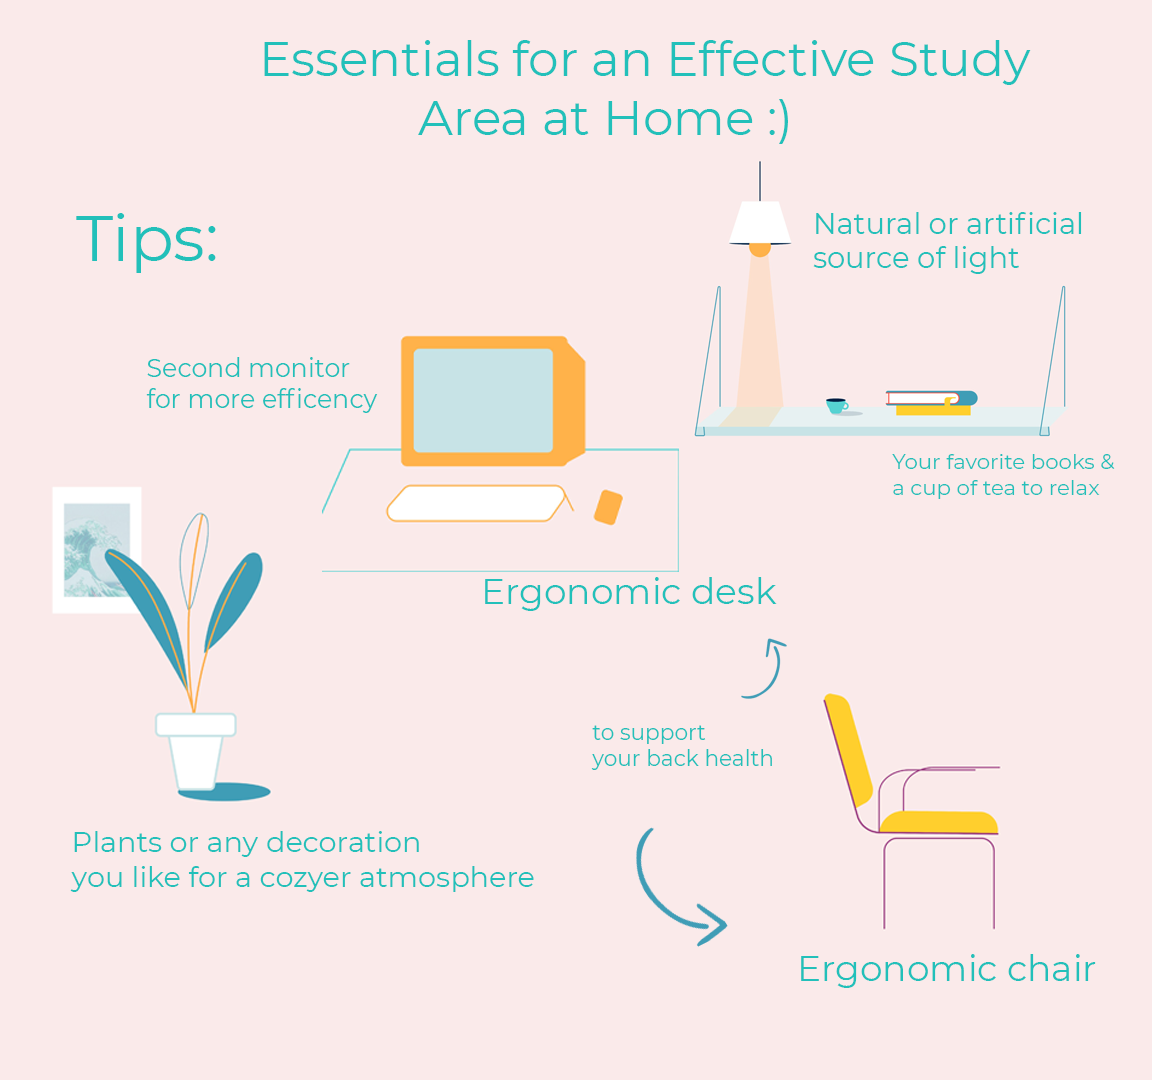
\includegraphics[width=1\columnwidth]{figures/leaflet.png}
  \caption{A sample informative leaflet created by our team in cooperation with Anna Scassillo}~\label{fig:figure4}
\end{figure}

\subsection{Replacement of Social interaction}

Multiple participants have expressed an inner desire to talk about their motivational issues while studying in this new environment. We were impressed that different solutions for coping were applied by each participant, from simple \emph{Zoom} study sessions, to potentially illegal (depending on the country) group lecture viewings that broke social distancing restrictions. Issue is that even with these make-shift solutions, lectures, class presentations and general group work are still much harder to occur under social isolation and current technological solutions are heavily lacking. Although, there are current projects such as VReddo \cite{vreddo_2020} that try to overcome this problem in the educational sector by providing Virtual Reality classroom equipment and software. While a solution like this can be quite expensive, especially for a university such as Vienna University of Technology that has such a large number of students registered, we would argue that it could be used to improve diploma presentations or classes with a small number of students.

Sadly, for now we would argue that there is no proper replacement for the in-class lecture experience, and most likely students will continue to feel a setback in their studies due to the continuous lack of interactivity that current IT solutions fail to overcome.

\section{Conclusions and Future Work}

This conference paper looked at the differences in students' study situations and at-home study spaces during the current pandemic of COVID-19. To protect society from the virus, the university has transformed teaching into a distance-adapted solution in the students' homes. This creates new challenges for all students, however, the challenges are different depending on their individual living situation. 

The research has shown that there is a deterioration in motivation due to the sustained distance learning. This places demands on students' inner motivation, which is a decisive factor in how the studies proceed. Although many students have good technical equipment in the form of computers and mobile phones with cameras, many students have nevertheless updated their equipment to some degree during the pandemic. As the individual circumstances of our participants' lives vary, it is not possible in this study to generalize the equipment gap, however, dual screens and touch-pads have been a prominent interest. We have identified simple changes a student could make to their at-home study environment that would improve the effectiveness of sustained distance-learning. Consequently, the university studies have a greater chance of success, despite the circumstances, as the students adapt to the new learning format. 

There is also a health risk that studies in the home office will cause ergonomic problems such as back pain, as the furniture in the home office may not offer the same comfort and support as the furniture at the university. There were also complaints of eye strain from inadequate lighting and from staring at a screen for too many hours. In many situations, the home office is in the same room as the student's bedroom. One solution is to move the desk closer to a window. This has the added benefit of helping the eyes rest as they focus on objects outside of the window, and to improve the student's mood and motivation. If this is not possible, a bright desk lamp or a standing lamp may be used. Additionally, if a student cannot afford a chair designed to support one for prolonged sitting, they can use lumbar supporting cushions as a backrest with their existing chair. 

As the pandemic experience influenced the way studies are carried out and brought with it a process of digitalization in the educational field, we believe that in the future a new alternative for studying may appear. A mix between having access to online courses and resources with the ability to join on-site laboratories and seminars, may offer more flexibility towards studies and may be a better solution for both students and teachers for organizing their schedule accordingly. Future research can be carried out focusing on the evolution of the environment at home in order to support the hybrid solution, and how having access to some of the university facilities and occasional social interaction can increase motivation.

Future research on the motivation of students engaged in distance learning studies, but not in a context of a pandemic, would also represent a major interest. Social interaction and collaboration are important values developed in the academic life and they were severely affected by the current situation by the regulations that are in place in nearly every country. Therefore, a further study that focuses on the motivation of individuals performing distance learning, but without any restriction on their personal life and with the possibility of meeting outside the university campus, would bring value to understand the necessity of academic social life.

Finally, we would like to point out that there is still a lack of awareness of how to carry out university studies in a distance-adapted format. According to our analysis, this has been overlooked due to the pandemic as well as the usual study workload that students have to complete. There are also financial reasons a student may not be able to create an "optimal" home-office. However, simple solutions can be found. We propose educational institutions to inform students about possible enhancements that they can implement in order to improve their home study environment. 


\section{Acknowledgments}
We thank all of our interview participants for taking the time from their studies and work in order to help us with this assignment. Thank you to Anna Scassillo for providing us with the amazing drawings used to create the informational leaflet. Thank you to Vienna University of Technology for giving us access to the needed tools in order to prepare this assignment, and of course to our supervisors for offering us guidance along the way.

% REFERENCES FORMAT
% References must be the same font size as other body text.
\bibliographystyle{SIGCHI-Reference-Format}
\bibliography{references}

\end{document}

%%% Local Variables:
%%% mode: latex
%%% TeX-master: t
%%% End:
